\section{Приложение математического\\моделирования для исследования\\экономических процессов}

В экономической части настоящей работы будет рассмотрена ранняя \textbf{модель капитализации Калецкого (Kalecki)}. Данная модель \--- одно из первых распространенных приложений дифференциальных уравнений с запаздыванием. Впервые описание данной модели самим Калецким было представлено в работе \cite{bib:Kalecki}.

\subsection{Основное макроэкономическое тождество}

Исходым допущением в модели Калецкого является выполнение \textbf{основного макроэкономического тождества}:

\begin{equation}
Y = C + I + A,
\end{equation}

где

\begin{enumerate}
\item $Y$ \--- совокупный доход (часто в его качестве рассматривается \textbf{валовый национальный продукт}(ВНП)),
\item $C = C_a + C_i$ \--- сумма интенсивностей автономного и индуцированного потребления,
\item $C_i = c Y$ \--- индуцированное потребление (т.е часть расходов, обусловленная изменением уровня располагаемого дохода $Y$),
\item $C_a$ \--- автономное потребление (т.е. часть расходов, постоянная вне зависимости от величины доходов $Y$),
\item $I = I_a + I_i$ \--- совокупные инвестиции,
\item $I_i = s Y$ \--- индуцированные инвестиции,
\item $I_a$ \--- автономные инвестиции,
\item $c+s=1, c>0, s>0$.
\end{enumerate}

Оно отражает равенство дохода и совокупных расходов (а значит, истинно только для \textbf{замкнутной экономической системы}).

\subsection{Вывод дифференциального уравнения с запаздыванием}

Пусть $K(t)$ \--- объем доступного капитала. Его динамику можно рассчитать следующим образом в силу запаздывания реакции системы на новый капитал:

\begin{equation}
K'(t + \tau) = a s Y(t) - b K(t) + \epsilon(t), \quad 0 < a < 1, b > 0,
\end{equation}

$\epsilon(t)$ \--- невязка.

Инвестиции $I(t)$ \--- изменение доступного капитала в атомарный период времени:

\begin{equation}
I(t) \dfrac{1}{\tau} \left( K(t+\tau) - K(t) \right)
\end{equation}

Далее

\begin{equation}
Y(t) = {underbrace{(1-s)) Y(t)}_{C_a(t)}}_{C(t)} + I(t) + A(t)
\end{equation}

\begin{equation}
Y(t) = \dfrac{1}{s} \left( I(t) + A(t) + C_a(t) \right)
\end{equation}

\begin{equation}
Y(t) = \dfrac{1}{s \tau} \left( K(t+\tau) - K(t) \right) + \dfrac{1}{s} \left( A(t) + C_a(t) \right)
\end{equation}

Таким образом,

\begin{equation}
K'(t + \tau) = a \dfrac{1}{\tau} \left( K(t+\tau) - K(t) \right) + a \left( A(t) + C_a(t) \right) - bK(t) + \epsilon(t)
\end{equation}

Наконец, перепишем уравнение в виде:

\begin{equation}\label{eq:Kalecki}
K'(t) - \dfrac{a}{\tau} K(t) + \left( \dfrac{a}{\tau} + b \right) K(t-\tau) = a (A(t-\tau) + C_a(t-\tau) + \epsilon(t-\tau))
\end{equation}

\subsection{Устойчивость уравнения Калецкого}

Для уравнения с запаздывваниям

\begin{equation}
\dot{x}(t) + a_1 x(t) + b_1 x(t-\tau) = 0
\end{equation}

было получено необходимое условие его асимптотической устойчивости (см, например, \cite{bib:Elsgoltz-Norkin}, с.133):

\begin{equation}
0 \leq \tau \dfrac{arccos \left( -\frac{a_1}{b_1} \right)}{\sqrt{b_1^2-a_1^2}}
\end{equation}

В терминах уравнения (\ref{eq:Kalecki}) получим:

\begin{equation}
0 \leq \tau < \dfrac{\tau \text{ } arccos \left( \frac{a}{a + b \tau} \right) }{\sqrt{b \tau (b \tau + 2a)}}
\end{equation}

\begin{equation}\label{eq:Kalecki-stab}
arccos \left( \frac{a}{a + b \tau} \right) > \sqrt{b \tau (b \tau + 2a)}
\end{equation}

Значения $a$, $b$, $\tau$ предполагаются известными, а значит, можно на основе проверки данного неравентсва судить об устойчивости всей модели.

\subsection{Пояснения}\label{sec:what}

Устойчивость модели Калецкого и характер отражаемых ею колебательных процессов зависят от значения коэффициентов $a$, $b$ в уравнении реакции системы. Коэффициент $a$ выражает \textbf{реакцию инвестиционных решений на доход} $Y(t)$, $b$ \--- \textbf{реакцию инвестиционных решений на запасы наличного основного капитала} $K(t)$. На основе статических данных на примере США на 1909-1918 гг. Калецкий провел пробную оценку значений коэффициентов a и b. Он определил, что $a=0.95$, $b=0.12$, причем $\tau$ \--- 1 год. Также он произвел оценку для США 1929-1940 гг. и получил $a=0.7$, $b=0.12$ c тем же периодом конъюктуры. Отметим, что в условиях кризиса параметр $a$ обычно минимален, а в условиях роста экономики после рецессии достигает своих максимальных значений. Это свидетельствует о неготовности предпринимателей совершать крупные инвестиции в будующее во время кризиса, и, наоборот, \--- об инвестиционном буме молодой экономики, показатель ВНП которой возрастает.

\newpage

\subsection{Примеры применения модели для моделирования процессов макроэкономики}

В данной части работы изобразим решения уравнений Калецкого в расмотренных им случаях, приведенных в пояснении к модели [\ref{sec:what}].

Для простоты примем $A=0$, $C_a=10$, $\epsilon=0$, $K(t)=1$, $-\tau \leq t \leq 0$.

\subsubsection{При $a=0.95$, $b=0.12$, $\tau=1$}

\begin{figure}[h]
\begin{center}
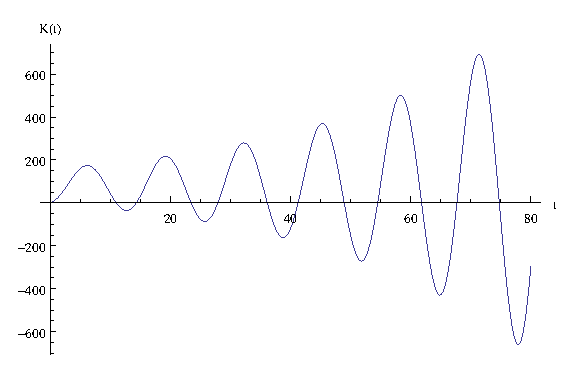
\includegraphics[width=0.65\textwidth]{./4_economics/unstable.eps}
\end{center}
\caption{График решения уравнения Калецкого при $a=0.95$, $b=0.12$, $\tau=1$}
\end{figure}

\begin{equation}\label{eq:Kalecki-stab}
arccos \left( \frac{0.95}{0.95 + 0.12} \right) \approx 0.478144 \leq 0.492341 \approx \sqrt{0.12 (0.12 + 2 \dot 0.95)}
\end{equation}

\subsubsection{При $a=0.7$, $b=0.12$, $\tau=1$}

\begin{figure}[h]
\begin{center}
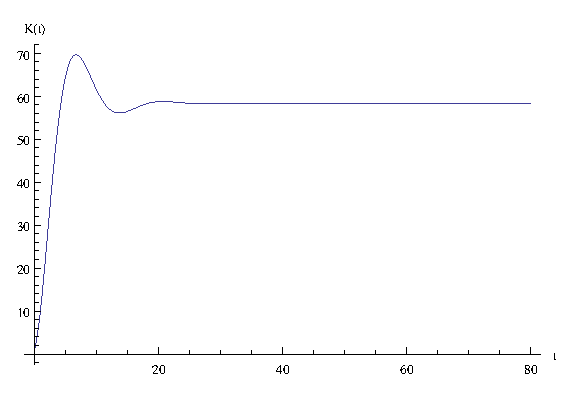
\includegraphics[width=0.65\textwidth]{./4_economics/stable.eps}
\end{center}
\caption{График решения уравнения Калецкого при $a=0.7$, $b=0.12$, $\tau=1$}
\end{figure}

\begin{equation}\label{eq:Kalecki-stab}
arccos \left( \frac{0.7}{0.7 + 0.12} \right) \approx 0.547827 > 0.427083 \approx \sqrt{0.12 (0.12 + 2 \dot 0.7)}
\end{equation}

\subsection{Вывод}

Таким образом, модель Калецкого описывает \textbf{процесс простого воспроизвоства}, которому соответсвуют либо колебания с возрастающей амплитудой, свидетельствующие о неустойчивости макроэкономике в исследуемый период, либо подавляемые колебания, соответствующие эмпирически установленному циклу хозяйственной конъюктуры.
